\documentclass[12pt]{article}
\usepackage[utf8]{inputenc}
\usepackage{graphicx}
\usepackage{parskip} 
\graphicspath{ {images/} }
\title{Text classification using the semi-supervised methods}
\author{Michał Filek}
\date{June 2020}

\begin{document}

\maketitle
% this line is a comment
% ABSTRACT
\begin{abstract}
This is a simple paragraph at the beginning of the 
document. A brief introduction about the main subject.
\end{abstract}

\tableofcontents


\section{Introduction}
\begin{figure}[h]
    \centering
    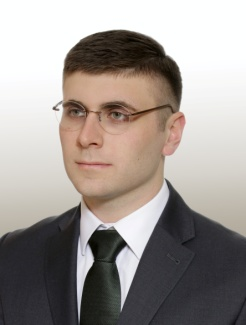
\includegraphics[width=0.25\textwidth]{photo.jpg}
    \caption{a nice plot}
    \label{fig:photo}
\end{figure}

As you can see in the figure \ref{fig:photo}, the 
function grows near 0. Also, in the page \pageref{fig:photo} 
is the same example.

\begin{itemize}
  \item The individual entries are indicated with a black dot, a so-called bullet.
  \item The text in the entries may be of any length.
\end{itemize}

\begin{enumerate}
  \item This is the first entry in our list
  \item The list numbers increase with each entry we add
\end{enumerate}

In physics, the mass-energy equivalence is stated 
by the equation $E=mc^2$, discovered in 1905 by Albert Einstein.

The mass-energy equivalence is described by the famous equation
\[ E=mc^2 \]
discovered in 1905 by Albert Einstein. 
In natural units ($c = 1$), the formula expresses the identity
\begin{equation}
E=m
\end{equation}




\section{Machine Learning basis}


This is the first section.

Lorem  ipsum  dolor  sit  amet,  consectetuer  adipiscing  
elit.   Etiam  lobortisfacilisis sem.  Nullam nec mi et 
neque pharetra sollicitudin.  Praesent imperdietmi nec ante. 
Donec ullamcorper, felis non sodales...



\subsection{Machine Learning Paradigms}
bla bla bla there are many, but three main

\subsubsection{Supervised Learning}
there are regression and classification - it will be discussed only classification
\subsubsection{Unsupervised Learning}
\subsubsection{Reinforcment Learning}

\subsection{Basic Asumptions}
\subsection{Classification}
\subsubsection{Geneartive Models}
\subsubsection{Discriminative Models}
\subsection{Loss Function}
\subsubsection{MAP}
\subsubsection{MLE}
\subsection{Overfitting, Underfitting, capacity}
\subsection{Regularization}
\subsubsection{Weight Decay}
\subsubsection{Dropout}
\subsubsection{Data Augmentation}

\section{Neural Networks}
    \subsection{Multilayer Perceptrons Networks}
    \subsection{Convolutional Networks}
        \subsubsection{On text}
    \subsection{Recurrent Networks}
        \subsubsection{LSTMs}
    \subsection{Attention Mechanism}

\section{Natural Language Processing}
    \subsection{Brief history of NLP}
    language models, pretrained self supervised representation learning
    pretraining
    \subsection{n-gram representations}
    \subsection{continues representations}
        \subsubsection{Feed Forward NNLM}
        \subsubsection{Word2Vec}
        \subsubsection{FastText}
        sfsafdsafdsf
        
        \subsubsection{BERT}
        
\section{Semi-supervised Learning}
        \subsection{Semi-supervised Learning Assumptions}
        \subsection{Semi-supervised Learning methods}
            \subsubsection{Entropy Minimization}
            \subsubsection{Label Propagation}
            \subsubsection{Self training}
            \subsubsection{Consistency Training}
                describe regularization and perturbations and transformations, ladder network
        \subsection{Brief history of Consistency Regularization}
             \subsubsection{II model, temporal ensambling}
             \subsubsection{Mean Teacher}
             \subsubsection{VAT}
             \subsubsection{MIXMATCH}
             \subsubsection{REMIXMATCH}
             \subsubsection{UDA}
             \subsubsection{FixMatch}
             
\section{Experiments}
    \subsection{Realistic Evaluation}
    \subsection{Experiment Settings}
    \subsection{Ablation Studies}

\section{Conclusions and Future Works}
\section{Acknowledgments}
\section{References}



            






        




        




\section{Unnumbered Section}
Lorem ipsum dolor sit amet, consectetuer adipiscing elit.  
Etiam lobortis facilisissem

\begin{center}
 \begin{tabular}{||c c c c||} 
 \hline
 Col1 & Col2 & Col2 & Col3 \\ [0.5ex] 
 \hline\hline
 1 & 6 & 87837 & 787 \\ 
 \hline
 2 & 7 & 78 & 5415 \\
 \hline
 3 & 545 & 778 & 7507 \\
 \hline
 4 & 545 & 18744 & 7560 \\
 \hline
 5 & 88 & 788 & 6344 \\ [1ex] 
 \hline
\end{tabular}
\end{center}

\end{document}

